%\documentclass[11pt]{article}
%\usepackage{fullpage}
%\usepackage{graphicx}

%\begin{document}
In this section, the Alloy model is given. Using it, some of the features of the system are specified and explained in more details, with the focus being on the constraints:
\begin{itemize}
\item The organizer must create a "valid" competition: track with well-defined start and finish, well-defined intermediate stages, maximum number of stages is 10 (track's lenght of a run can be at max 50km).
\item Data sent to a third party must be part of or data of a specific individual or an anonymous group of at least 1000 subjects.
\item Generic users that are in a specific individual data survey will recieve a notification.
\item If at least one between BPM, blood pressure or glucose of a user will exceed minimum or maximum threshold, an Emergency dispatcher will recieve a warning (CallAmbulanceWarning), that will be used to send an ambulance to the user who needs help.
\item Users can participate to competitions and can be marked as disqualified by the organizer, and if an athlete is marked as disqualified he will not appear in the list of active runners.
\end{itemize}

In the model of Alloy described we have simplified the numerical values, for example the races can be a maximum of 7 (= 50km) and there con be a maximum of 7 stages (= 10), the position, coordX and coordY, are limited respectively between -3 and 3, between -6 and 6. The number of people in a survey that indicates that it can be an anonymized data survey is 2 (= 1000). BPM, blood pressure, glucose are represented by values between 1 and 6, so it is for thresholds. 
\subsection{Alloy model}
\lstinputlisting[language=alloy]{sections/trackMe.als}
\clearpage
\subsection{World generated}
Figure 15 shows a possible world generated with the run of the second pred (run showAutomatedSOS). On top of the image there is an "OpenRun" and at the bottom (under Track) there is the track's lenght (7).

\begin{figure}[h!] \ContinuedFloat
\centering
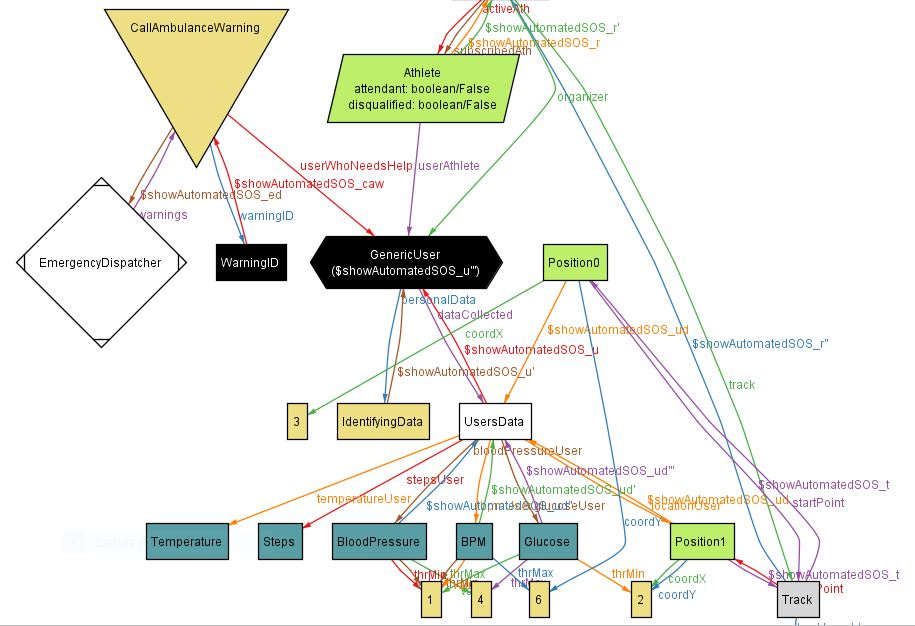
\includegraphics[scale=0.75]{sections/alloy_images/worldGenerated.JPG} \newline
\captionof{figure}{World generated}
\end{figure}
\clearpage
\subsection{Alloy results}
These are the results produced by the code shown above.

\begin{figure}[h!] \ContinuedFloat
\centering
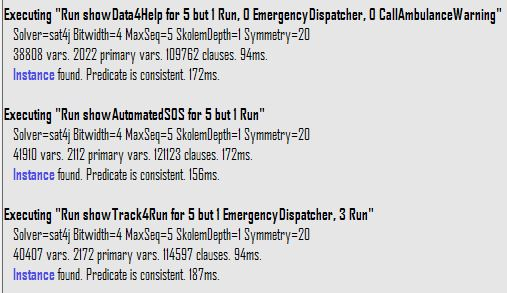
\includegraphics[scale=1]{sections/alloy_images/runResults.JPG} \newline
\captionof{figure}{Alloy results}
\end{figure}

%\end{document}